\documentclass[xcolor=dvipsnames]{beamer}
\usepackage{lmodern}
\usepackage[T1]{fontenc}
\usepackage[english]{babel}
\usepackage[utf8]{inputenc}

\usepackage{manfnt}
\usepackage{wasysym}
\usepackage{listings}
\usepackage{graphicx}
\usepackage{url}
\usepackage{ulem}
\usepackage{marvosym}
\usepackage{skull}
\usepackage{proof}
\usepackage{array}
\usepackage{colortbl}
\usepackage{xspace}
\setbeamertemplate{navigation symbols}{}

\title[]{{\bf Practical Concurrency Testing}}
\subtitle[]{or, \\ How I Learned to Stop Worrying and Love the Exponential Explosion}
\author[]{Ben Blum \texttt{(bblum@cs.cmu.edu)}}

\institute[]{Carnegie Mellon University}
\date[]{2018, October 17}

\setbeamertemplate{footline}{\hspace*{.5cm}\scriptsize{\insertauthor\hspace*{50pt} \hfill\insertframenumber\hspace*{.5cm}}} 

\usecolortheme{seahorse}
\usecolortheme{rose}
\useoutertheme{infolines}

\usecolortheme[named=ForestGreen]{structure}

\newcommand\noob{\mathsf{noob}}
\newcommand\gibs{\mathsf{gibs}}
\newcommand\dps{\mathsf{dps}}
\newcommand\squig\rightsquigarrow
\newcommand\Coloneqq{\mathrel{\mathop{::}}=}
\newcommand\dmg{\text{\Laserbeam}}
\newcommand\delter\delta
\newcommand\alpher\alpha
\newcommand\defnor{\text{ }|\text{ }}

\newcommand\pimp{\mathop{\supset}}
\newcommand\pand{\mathop{\wedge}}
\newcommand\por{\mathop{\vee}}
\newcommand\ptrue{\top}
\newcommand\pfalse{\bot}

\newcommand\hilight[2]{\color{#1}#2\color{black}}
\definecolor{olivegreen}{RGB}{0,127,0}

\begin{document}
\renewcommand{\inserttotalframenumber}{39}
\normalem
\begin{frame}
	\titlepage
\end{frame}

%%%%%%%%%%%%%%%%%%%%%%%%%%%%%%%%%%%%%%%%%%%%%%%%%%%%%%%%%%%%%%%%%%%%%%%%%%%%%%%%
%%%%%%%%%%%%%%%%%%%%%%%%%%%%%%%%%%%%%%%%%%%%%%%%%%%%%%%%%%%%%%%%%%%%%%%%%%%%%%%%
%%%%%%%%%%%%%%%%%%%%%%%%%%%%%%%%%%%%%%%%%%%%%%%%%%%%%%%%%%%%%%%%%%%%%%%%%%%%%%%%

\newcommand\linegap{\vspace{0.2in}}
\newcommand\breakslide[1]{\begin{frame}{} \begin{center} #1 \end{center} \end{frame}}

\section{Part 0}
\subsection{Motivation}

\begin{frame}{Concurrency!}
	\begin{center}
	\begin{tabular}{ll}
		Initially \texttt{x = 0;} \\
		\\
		{\bf Thread 1} & {\bf Thread 2} \\
		\\
		\texttt{\hilight{orange}{mutex\_lock}(m);}      & \texttt{atomic\_xadd(\&x, 1);} \\
		\texttt{x++;}				   & \texttt{\hilight{olivegreen}{yield}();} \\
		\texttt{\hilight{blue}{mutex\_unlock}(m);}      & \texttt{atomic\_xadd(\&x, 1);} \\
		\texttt{assert(x >= 1);}			& \texttt{assert(x >= 2);} \\
		\\
		\\
		\\
		\\
		\\
	\end{tabular}
	\end{center}
\end{frame}
\begin{frame}{Concurrency!}
	\begin{center}
	\begin{tabular}{ll}
		Initially \texttt{x = 0;} \\
		\\
		{\bf Thread 1} & {\bf Thread 2} \\
		\\
		\texttt{\hilight{orange}{mutex\_lock}(m);} \\
		\texttt{int tmp = x;} \\
								& \texttt{atomic\_xadd(\&x, 1);} \\
								& \texttt{\hilight{olivegreen}{yield}();} \\
								& \texttt{atomic\_xadd(\&x, 1);} \\
		\texttt{x = tmp + 1;} \\
								& \texttt{\hilight{red}{assert(x >= 2);}} \\
		\texttt{\hilight{blue}{mutex\_unlock}(m);} \\
		\texttt{assert(x >= 1);}
	\end{tabular}
	\end{center}
\end{frame}

\begin{frame}{Stateless Model Checking}
	Stateless Model Checking {\em [Godefroid '97]} (MC)
	\begin{itemize}
		\item Test framework controls thread scheduling
		\item Each test iteration, test a different interleaving
		\item Goal: Exhaustively check all possible program behaviours
	\end{itemize}
	\pause
	\linegap

	\begin{center}
		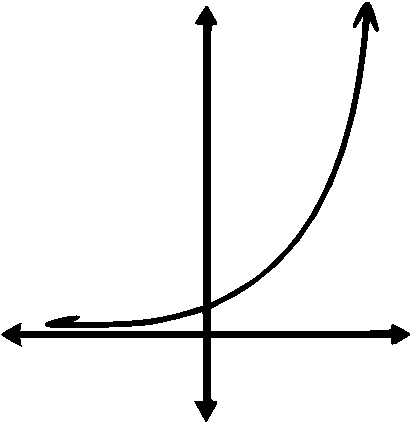
\includegraphics[width=0.25\textwidth]{../../oopsla/exponential-curve.pdf}
	\end{center}
\end{frame}

\begin{frame}{State Space Example}
	\begin{center}
		\includegraphics[width=0.96\textwidth]{../../oopsla/tree-maximal-only.pdf}
	\end{center}
	\linegap

	Possible interleavings represented as a tree
	\begin{itemize}
		\item Node: Intermediate execution state
		\item Edge: State transition from executing a thread
	\end{itemize}
	\linegap

	State space size depends on which {\bf preemption points} are used.
\end{frame}

\begin{frame}{Challenges} %\& Existing Coping Techniques}
	Unpredictable state space explosion
	\begin{itemize}
		\item Equivalence reductions: DPOR {\em [Flanagan '05]}, MCR {\em [Huang '15]}
		\item Heuristic search ordering: ICB {\em [Musuvathi '08]}, PCT {\em [Burckhardt '10]}
		\item There will always be a {\bf bigger test case}!
	\end{itemize}
	\pause
	\linegap

	Too much manual intervention for non-expert use
	\begin{itemize}
		\item Manual kernel annotations: Landslide {\em [Blum '12]} {\tiny that's me!}
			% TODO: smth about choosing pps?
		\item State space size estimation {\em [Simsa '12]}
			% TODO change this bullet pt to be more explicitly about 
		\item Widespread adoption requires {\bf fully automated instrumentation}!
	\end{itemize}
	\pause
	\linegap

	Limited sources of nondeterminism
	\begin{itemize}
		\item Timer-driven schedule nondeterminism (all prior work)
		\item Weak memory nondeterminism {\em [Zhang '15]}
		\item Event-driven applications {\em [Jensen '15]}
		\item {\bf Hardware transactional memory}?
	\end{itemize}
\end{frame}

%\begin{frame}{overview of state of art}
%	\begin{itemize}
%		\item so like, you got all this threads, right?
%		\item n then you just make em go any which way
%		\item see what all bugs come out
%	\end{itemize}
%\end{frame}

\begin{frame}{Thesis Statement}
	% data race pps (as well as txn equivalence)
	Combining both theoretically-founded automatic reduction techniques
	% iterative deepening
	% (say smth like: "landslide also has a wealth of other user-tunable heuristics
	% for expert users, which you can read about in the document; for this talk i will focus just on the CPU budget thing")
	% XXX: need to prepare for the question -- "what evidence do you have that users actually want this cpu budget stuff",
	% ",or, that it helps vs just running something unlimited vs a normal icb test"
	% (well, for the 2nd half of the Q, i can talk about how ID outperforms ICB on verficiations)
	and user-informed heuristic ones,
	stateless model checking can sufficiently mitigate exponential explosion to be
	% education
	a practical testing technique for inexperienced users
	% htm
	% TODO: this last part you just added for this talk; does the thesis version of the statmeent need to include too?
	and real-world programs alike.
\end{frame}

\definecolor{gray}{RGB}{128,128,128}

\begin{frame}{Thesis Statement}
	The Iterative Deepening algorithm makes MC appropriate for both educational and real-world programs.
	\vspace{4.14em}

	Ad-hoc synchronization heuristics make MC accessible to student programmers.
	\vspace{4.14em}

	A new transactional concurrency model keeps MC applicable to the latest real-world techniques.
	\vspace{4.14em}
\end{frame}
\begin{frame}{Outline}
	\hilight{gray}{The Iterative Deepening algorithm makes MC appropriate for both educational and real-world programs.} \\
	\begin{itemize}
		\item {\bf Quicksand and Iterative Deepening}
		\begin{itemize}
			\item Algorithm overview \& data-race preemption points
			\item Verification \& experimental results
		\end{itemize}
	\end{itemize}
	\hilight{gray}{Ad-hoc synchronization heuristics make MC accessible to student programmers.} \\
	\begin{itemize}
		\item {\bf Educational use}
		\begin{itemize}
			\item Pebbles \& 15-410 user study
			\item Pintos \& upcoming plans
		\end{itemize}
	\end{itemize}

	\hilight{gray}{A new transactional concurrency model keeps MC applicable to the latest real-world techniques.} \\
	\begin{itemize}
		\item {\bf Transactional memory}
		\begin{itemize}
			\item Example \& challenges
			\item Equivalence \& failure injection
		\end{itemize}
	\end{itemize}
\end{frame}

%\begin{frame}{Outline}
%	guess i should outline my talk huh
%\end{frame}


%%%%%%%%%%%%%%%%%%%%%%%%%%%%%%%%%%%%%%%%%%%%%%%%%%%%%%%%%%%%%%%%%%%%%%%%%%%%%%%%
%%%%%%%%%%%%%%%%%%%%%%%%%%%%%%%%%%%%%%%%%%%%%%%%%%%%%%%%%%%%%%%%%%%%%%%%%%%%%%%%
%%%%%%%%%%%%%%%%%%%%%%%%%%%%%%%%%%%%%%%%%%%%%%%%%%%%%%%%%%%%%%%%%%%%%%%%%%%%%%%%

\section{Part 1}
\subsection{Quicksand}

\breakslide{\Large Quicksand}

\begin{frame}{Preemption Points}
	The burning question: ``Which {\bf preemption points} (PPs) are important?''
	\linegap

	State space of interleavings is {\em parameterized} by PPs.
	\begin{itemize}
		\item Too few PPs: Many bugs will go undetected
		\item Preempt everywhere: Completion is often infeasible % say: "for some programs"
	\end{itemize}
	\linegap

	Prior model checkers hard-code a fixed set of PPs, committing to one state space in advance.
	% say: "...then attempt to cope with the resulting exponentially sized problem, however big it may be"
\end{frame}

\begin{frame}{Example (Revisited)}
	\begin{center}
	\begin{tabular}{ll}
		Initially \texttt{x = 0;} \\
		\\
		{\bf Thread 1} & {\bf Thread 2} \\
		\\
		\texttt{\hilight{orange}{mutex\_lock}(m);} \\
		\texttt{int tmp = x;} \\
								& \texttt{atomic\_xadd(\&x, 1);} \\
								& \texttt{\hilight{olivegreen}{yield}();} \\
								& \texttt{atomic\_xadd(\&x, 1);} \\
		\texttt{x = tmp + 1;} \\
								& \texttt{\hilight{red}{assert(x >= 2);}} \\
		\texttt{\hilight{blue}{mutex\_unlock}(m);} \\
		\texttt{assert(x >= 1);}
	\end{tabular}
	\end{center}
\end{frame}

\begin{frame}{State Space (Revisited)}
	\begin{center}
		\includegraphics[width=0.96\textwidth]{../../oopsla/tree-maximal-only.pdf}
		\linegap

		None of these branches contain the necessary preemption!
		\linegap

		A {\bf data-race preemption point} is required to find the bug.
	\end{center}
\end{frame}

\begin{frame}{Data Race Analysis}
	A {\bf data race} is a pair of memory accesses between two threads, where:
	\begin{itemize}
		\item At least one of the accesses is a write
		\item The threads are not holding the same mutex
		\item One access {\em happens-before} the other
			(e.g., no \texttt{cond\_signal()} in between)
	\end{itemize}
	\pause
	\linegap

	Two flavors
	\begin{itemize}
		\item {\bf Pure HB}: Whether accesses were {\em observed simultaneously}, false-negative prone
			{\em [Lamport '78]}
		\item {\bf Limited HB}: Whether threads {\em could be reordered}, false-positive prone
			{\em [O'Callahan '03]}
	\end{itemize}
\end{frame}

\begin{frame}{Iterative Deepening (in Pictures)}
	\begin{center}
	\vspace{-0.88em}
	\includegraphics[width=0.86\textwidth]{../../oopsla/dr-jobs-1.pdf}
	\end{center}
\end{frame}
\begin{frame}{Iterative Deepening (in Pictures)}
	\begin{center}
	\vspace{-0.88em}
	\includegraphics[width=0.86\textwidth]{../../oopsla/dr-jobs-2.pdf}
	\end{center}
\end{frame}
\begin{frame}{Iterative Deepening (in Pictures)}
	\begin{center}
	\vspace{-0.88em}
	\includegraphics[width=0.86\textwidth]{../../oopsla/dr-jobs-3.pdf}
	\end{center}
\end{frame}
\begin{frame}{Iterative Deepening (in Pictures)}
	\begin{center}
	\vspace{-0.88em}
	\includegraphics[width=0.86\textwidth]{../../oopsla/dr-jobs-4.pdf}
	\end{center}
\end{frame}

% TODO put a pict of mario-man, i.e maximal state space

\begin{frame}{Total Verification}
	\textbf{Convergence theorem:} Testing maximal state space, after detecting all data races, $\equiv$ preempting everywhere!
	\begin{itemize}
		\item Insight: $\forall$ arbitrary buggy interleaving, $\exists$ equivalent interleaving % say 'under DPOR' i guess?
			using only sync/data-race PPs, \& Quicksand will eventually reach it.
	\end{itemize}
	\linegap

	Hence, Iterative Deepening provides ``best of both worlds'':
	\begin{itemize}
		\item Provides total safety guarantee for small tests
		\item Finds bugs quickly for large tests when completion is infeasible
	\end{itemize}
\end{frame}

\begin{frame}{Evaluation}
	79 ``P2'' thread libraries from CMU, 78 ``Pintos'' kernels from U. Chicago \& Stanford
	\linegap

	%629 pairs of \{P2 or Pintos\} + test case
	629 pairs of P2 or Pintos + test case
	\linegap

	Each tested for 10 CPU-hours with
	\begin{itemize}
		\item Quicksand, finding data-race candidates with...
			\begin{itemize}
				\item ...``Pure'' Happens-Before analysis {\em [Lamport '78]}
				\item ...``Limited'' Happens-Before analysis {\em [O'Callahan '03]}
			\end{itemize}
		\item Stand-alone Landslide using ICB {\em [Musuvathi '08]}, preempting at...
			\begin{itemize}
				\item ...synchronization APIs only {\em [Simsa '10]}
				\item ...all shared memory accesses
					%{\em [Holzmann '97]} % not spin
					{\em [Yang '08]} % inspect
			\end{itemize}
	\end{itemize}
\end{frame}

\begin{frame}{Results - Bugs found}
	\begin{center}
		\includegraphics[width=0.8\textwidth]{../../oopsla/bugs-talk.pdf}
	\end{center}
\end{frame}
\begin{frame}{Results - Full verifications}
	\begin{center}
		\includegraphics[width=0.8\textwidth]{../../oopsla/verifs-talk.pdf}
	\end{center}
\end{frame}

\begin{frame}{Summary}
	Incorporate data-race analysis to add new PPs in a feedback loop
	\linegap

	Enough time to saturate \& test every data-race PP? Full verification
	\linegap

	Otherwise? Quicksand's heuristic search ordering finds bugs faster anyway
	\pause
	\linegap

	%Future work
	%\begin{itemize}
	%	\item Extend proof to weak memory
	%	\item Incorporate ICB in Quicksand
	%	\item Improve estimation accuracy
	%\end{itemize}
\end{frame}

%%%%%%%%%%%%%%%%%%%%%%%%%%%%%%%%%%%%%%%%%%%%%%%%%%%%%%%%%%%%%%%%%%%%%%%%%%%%%%%%
%%%%%%%%%%%%%%%%%%%%%%%%%%%%%%%%%%%%%%%%%%%%%%%%%%%%%%%%%%%%%%%%%%%%%%%%%%%%%%%%
%%%%%%%%%%%%%%%%%%%%%%%%%%%%%%%%%%%%%%%%%%%%%%%%%%%%%%%%%%%%%%%%%%%%%%%%%%%%%%%%

\section{Part 2}
\subsection{Education}

\breakslide{\Large Education}

\begin{frame}{Setting}
	CMU (15-410, S'15-S'18), PSU (CMPSC 473, S'18)
	\begin{itemize}
		\item Thread library (``P2'')
			\begin{itemize}
				\item POSIX-like userspace thread library %(also teams of 2)
				\item Reference ``Pebbles'' kernel provided
					% say: later they implement this in p3
				\item Fixed APIs $\rightarrow$ instrumentation can be automated
				\item Still needs heuristics to handle ad-hoc synchronization
			\end{itemize}
			% FIXME: need introduce p3 here?
	\end{itemize}
	\pause
	\linegap

	U. Chicago (CMSC 23000, F'17)
	\begin{itemize}
		\item Pintos %(``threads'' and ``userprog'')
		\begin{itemize}
			\item Basecode provides round-robin scheduler, synchronization, VM, loader
			\item ``threads'': Students implement priority scheduling, sleep
		%\end{itemize}
		%\linegap

		%\item Processes (``userprog'')
		%\begin{itemize}
				% fork is part of exec and the loader is already provided
			\item ``userprog'': UNIX-like process lifecycle
				%({\tt exec},
				({\tt exit}, {\tt wait})
			%\item File descriptor management ({\tt create}, {\tt remove}, {\tt open}, {\tt read}, ...)
				% filesys project is beyond scope of landslide
				% DONT say: the u chicago professor chose to discard the hard concurrency parts
				% DO say, if pressured: device driver concurrency would require more engineering,
				% so we chose to limit it to these two projex
		\end{itemize}
	\end{itemize}
\end{frame}

\begin{frame}{Instrumentation}
	% Unlike kernels [Blum '12], P2 can be......
	% TODO talk abt yield loops, 
	% compare to prior technique - delay abounding - which sucks bc (verify this by reading BPOR) it doesn't actually
	% wake up the other thread at the right time (using memory conflix)

	% pintos - bunch of gross patch stuff lmao
\end{frame}

% do even need this slide?
%\begin{frame}{Evaluation Questions}
%	asfda % TODO
%	% submit better projects?
%	% get better grades?
%	% like the experience?
%\end{frame}

\begin{frame}{Method}
	P2 (CMU + PSU)
	\begin{itemize}
		\item Guest lecture midway during project
		\item Landslide (+ Quicksand) provided to students with 6 test cases %and user guide
		\item Recorded code snapshots and bugs found each use (CMU only)
		\item Surveyed students on usability, false positives, etc.
	\end{itemize}
	\pause
	\linegap

	Pintos (U. Chicago)
	\begin{itemize}
		\item TA %(Kevin Zhao)
			ran Landslide on {\em threads} and {\em userprog} submissions
		\item Returned preemption traces to students after deadline
		\item Surveyed students on ease of debugging, etc.
	\end{itemize}
	% TODO: irb stuff in a bonus slide
\end{frame}

\begin{frame}{Results}
	Participation
	\begin{itemize}
		\item CMU: 103/177 students (7 semesters)
		\item PSU: 38/136 students (1 semester)
		\item U. Chicago: 4/21 students (1 semester)
	\end{itemize}
	\linegap

	Bug-finding
	\begin{itemize}
		\item CMU: 115 deterministic, 122 concurrency bugs in 75/103 P2s
		\item U. Chicago: 3 deterministic, 4 concurrency bugs in 3/4 kernels
		% \item Case study tej
	\end{itemize}
\end{frame}

\begin{frame}{Effect on Grades}
	Compared Landslide users' vs. non-users' submitted P2 grades...
	\begin{itemize}
		\item ``Does Landslide help students submit better projects?''
	\end{itemize}
	\linegap

	...as well as subsequent P3 (kernel) grades
	\begin{itemize}
		\item ``Does Landslide teach students lasting lessons about concurrency?''
	\end{itemize}
\end{frame}

\begin{frame}{Effect on Grades}
	\begin{center}
		\includegraphics[width=\textwidth]{../photo-of-ze-studence.pdf}
	\end{center}
\end{frame}

\begin{frame}{Effect on Grades}
	\begin{center}
		\includegraphics[width=\textwidth]{../photo-of-ze-studence-cdf.pdf}
	\end{center}
\end{frame}

\begin{frame}{Statistical Significance}
	Compared users' vs. non-users' grade distributions with k-sample Anderson-Darling {\em [Anderson, Darling '52]}
	\linegap

	Control 1: non-users from {\bf same semester}
	\begin{itemize}
		\item {\bf P2} grade distributions differ with $p = 0.036 < 0.05$
		\item {\bf P3} grade distributions differ with $p = 0.034 < 0.05$
			\pause
		\item Possible bias: stronger students volunteer for Landslide in first place
	\end{itemize}
	\pause
	\linegap

	Control 2: non-users from {\bf past semesters} (when Landslide not offered)
	\begin{itemize}
		\item {\bf P2} grade distributions differ with $p = 0.671$...
		\item {\bf P3} grade distributions differ with $p = 0.145$...
			\pause
		\item Possible bias: grading criteria may drift across semesters
			% FIXME does this bullet belong in this sub list
		\item Possible bias: maybe Landslide finds bugs the official tests don't
	\end{itemize}
\end{frame}

\begin{frame}{Survey}
	14(ish) questions, investigate both education \& happiness
	\begin{itemize}
		\item {\em Education:} Did Landslide help students learn more from P2?
		\item {\em Happiness:} Did Landslide help students save time/effort?
	\end{itemize}
	\linegap

	Self-report any false positives
	\begin{itemize}
		\item Landslide crashes aside, 3 FP bug reports, all simple bugs (now fixed)
			% nonexistent MAGIC_BREAK bc of different address space in shell
			% simultaneous landslides corrupt each other
			% invalid heap access when new_pages "too close"
		\item No FPs related to yield-loop/etc heuristics
	\end{itemize}
\end{frame}

\begin{frame}{Survey Results (educational value)}
	\begin{center}
		\includegraphics[width=\textwidth]{../survey6.pdf} % easier to diagnose?
	\end{center}
\end{frame}

\begin{frame}{Survey Results (happiness value)}
	\begin{center}
		\includegraphics[width=\textwidth]{../survey5.pdf} % easy to understand?
	\end{center}
\end{frame}

\begin{frame}{Survey Results (educational value)}
	\begin{center}
		\includegraphics[width=\textwidth]{../survey9.pdf} % 100 cpu hours
	\end{center}
\end{frame}

\begin{frame}{Survey Results (educational value)}
	\begin{center}
		\includegraphics[width=\textwidth]{../survey8.pdf} % learned to understand concurrency
	\end{center}
\end{frame}

\begin{frame}{Survey Results (happiness value)}
	\begin{center}
		\includegraphics[width=\textwidth]{../survey10.pdf} % recommend to friend
	\end{center}
\end{frame}

\begin{frame}{Summary}
	Landslide helps students find \& fix bugs during projects
	\begin{itemize}
		\item 73\% of CMU users found $\ge 1$ bug
		\item 56\% of CMU users fixed $\ge 1$ bug
		\item 34\% of CMU users fixed all found bugs
	\end{itemize}
	\linegap

	Effect on overall project grades: ???
	\begin{itemize}
		\item Compensating for experimental bias difficult w/human subjects...
	\end{itemize}
	\linegap

	Survey results showed students enlightenedly happy
	\linegap

	15-410 course staff now including Landslide in official grading :)
\end{frame}


%%%%%%%%%%%%%%%%%%%%%%%%%%%%%%%%%%%%%%%%%%%%%%%%%%%%%%%%%%%%%%%%%%%%%%%%%%%%%%%%
%%%%%%%%%%%%%%%%%%%%%%%%%%%%%%%%%%%%%%%%%%%%%%%%%%%%%%%%%%%%%%%%%%%%%%%%%%%%%%%%
%%%%%%%%%%%%%%%%%%%%%%%%%%%%%%%%%%%%%%%%%%%%%%%%%%%%%%%%%%%%%%%%%%%%%%%%%%%%%%%%

\section{Part 3}
\subsection{Transactional Memory}
\newcommand\xbegin{\texttt{\_xbegin()}\xspace}
\newcommand\xend{\texttt{\_xend()}\xspace}
\newcommand\xabort{\texttt{\_xabort()}\xspace}

\breakslide{\Large Transactional Memory}

\begin{frame}{Example}
	\begin{center}
		\begin{tabular}{l}
			\texttt{if ((status = \_xbegin()) == \_XBEGIN\_STARTED) \{} \\
			%\texttt{} \\
			%\texttt{} \\
			\texttt{~~~~foo++;} \\
			\texttt{~~~~\_xend();} \\
			\texttt{\} else \{}\\ %if (status != \_XABORT\_EXPLICIT) \{} \\
			\texttt{~~~~mutex\_lock(\&foo\_lock);} \\
			\texttt{~~~~foo++;} \\
			\texttt{~~~~mutex\_unlock(\&foo\_lock);} \\
			\texttt{\}} \\
		\end{tabular}
	\end{center}
\end{frame}

\begin{frame}{HTM Execution Semantics}
	Attempting a transaction
	\begin{itemize}
		\item Code between \xbegin and \xend is provisionally executed
		\item All writes kept in cache until \xend
		\item \xend commits changes atomically (w.r.t. other CPUs)
	\end{itemize}
	\pause
	\linegap

	Transaction failure
	\begin{itemize}
		\item Possible reasons:
			\begin{itemize}
				\item Memory conflict with another thread
				\item False sharing (conflict on same cache-line)
				\item Cache eviction, random interrupt, ...
			\end{itemize}
		\item Changes discarded, local state reverted, \xbegin returns failure
		\item {\tt else} branch runs some user-supplied backup plan
	\end{itemize}
\end{frame}

\begin{frame}{Model Checking Transactional Programs}
	What does it mean to MC a program?
	\begin{itemize}
		\item Capture all sites of nondeterminism as preemption points
		\item Control nondeterminism to force each possibility at each point
		\item (Identify equivalences to prune unnecessary preemption points)
	\end{itemize}
	\pause
	\linegap

	MCing a transactional program
	\begin{itemize}
		\item Simulate TM, interleaving transactions, rolling-back upon conflicts
			\begin{itemize}
				\item slow; invites state space explosion
			\end{itemize}
		\item Enforce atomicity via scheduler, anticipate aborts on every transaction
			%via analysis
			%\begin{itemize}
			%	\item (under HTM, all transactions might abort)
			%\end{itemize}
		\item Suffices to enumerate all {\em observationally-equivalent} schedules.
	\end{itemize}
\end{frame}

\begin{frame}{Concurrency model}
	What are a transactional program's {\em observable} behaviours?
	\begin{itemize}
		\item Transactional writes, if successful, appear atomically %to other threads
		\begin{itemize}
			\item Equivalent to a lock protecting that state
				% note that also inserting DR PPs within a transaction is not allowed
		\end{itemize}
			\pause
		\item Simultaneous transactions succeed only if no conflicts
		\begin{itemize}
			\item Equivalent
				%(modulo performance)
				to serialize independent transactions
		\end{itemize}
			\pause
		\item Failing transactions' effects rolled-back with no trace
		\begin{itemize}
			\item Treat each \xbegin as a failure injection point
		\end{itemize}
	\end{itemize}
\end{frame}

\begin{frame}{Failure Injection - 2 dimensions of concurrency}
	\begin{center}
		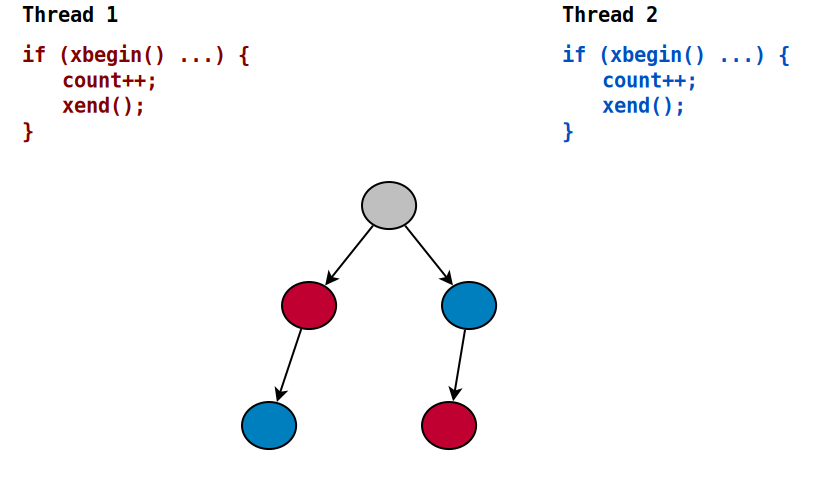
\includegraphics[width=\textwidth]{failure-injection-0.pdf}
	\end{center}
\end{frame}
\begin{frame}{Failure Injection - 2 dimensions of concurrency}
	\begin{center}
		\includegraphics[width=\textwidth]{failure-injection-2.pdf}
	\end{center}
\end{frame}

\begin{frame}{Deliverables}
	In the thesis, I will:
	\begin{itemize}
		\item Implement the HTM(-equivalent) concurrency model in Landslide
		\item Extend the model to support STM
		\item Prove equivalence to HTM/STM semantics % under MC
		\item Bugfind/verify a suite of unit tests \& real-world TM programs
	\end{itemize}
\end{frame}

%%%%%%%%%%%%%%%%%%%%%%%%%%%%%%%%%%%%%%%%%%%%%%%%%%%%%%%%%%%%%%%%%%%%%%%%%%%%%%%%
%%%%%%%%%%%%%%%%%%%%%%%%%%%%%%%%%%%%%%%%%%%%%%%%%%%%%%%%%%%%%%%%%%%%%%%%%%%%%%%%
%%%%%%%%%%%%%%%%%%%%%%%%%%%%%%%%%%%%%%%%%%%%%%%%%%%%%%%%%%%%%%%%%%%%%%%%%%%%%%%%

\section{End}

\breakslide{\Large Q\&A
%\linegap
%
%\begin{center}
%	\includegraphics[width=0.65\textwidth]{3word-questions.png}
%\end{center}
}

%%%%%%%%%%%%%%%%%%%%%%%%%%%%%%%%%%%%%%%%%%%%%%%%%%%%%%%%%%%%%%%%%%%%%%%%%%%%%%%%
%%%%%%%%%%%%%%%%%%%%%%%%%%%%%%%%%%%%%%%%%%%%%%%%%%%%%%%%%%%%%%%%%%%%%%%%%%%%%%%%
%%%%%%%%%%%%%%%%%%%%%%%%%%%%%%%%%%%%%%%%%%%%%%%%%%%%%%%%%%%%%%%%%%%%%%%%%%%%%%%%

\section{Bonus Slides}

\breakslide{\Large Bonus Slides}

\begin{frame}{15-410...}
	% TODO:
	% study of tej/etc specific bugs
	% list tests cases provided to studence & PSU-specific ones too
\end{frame}

\begin{frame}{HTM: Even more dimensions of nondeterminism}
	% The gotcha: When xbegin can fail, it can emit diff error codes, which depend on what happened within.
	\begin{center}
		\begin{tabular}{l}
			\texttt{if ((status = \_xbegin()) == \_XBEGIN\_STARTED) \{} \\
			\texttt{~~~~if (count < 100)}\\
			\texttt{~~~~~~~~\_xabort();} \\
			\texttt{~~~~count++;} \\
			\texttt{~~~~\_xend();} \\
			\texttt{\} else if (status != \_XABORT\_EXPLICIT) \{} \\
			\texttt{~~~~mutex\_lock(\&count\_lock);} \\
			\texttt{~~~~count++;} \\
			\texttt{~~~~mutex\_unlock(\&count\_lock);} \\
			\texttt{\}} \\
		\end{tabular}
	\end{center}
	\linegap

	\xbegin can fail with multiple possible error codes
	\begin{itemize}
		\item MC will identify on-the-fly when (e.g.) {\tt \_XABORT\_EXPLICIT} is possible
		\item Treat such transactions as having multiple failure injection possibilities
		\item Future work: dataflow analysis to identify when failure reason never used
	\end{itemize}
\end{frame}

\begin{frame}{HTM: Possible \xabort error codes}
	From GCC 4.8.2 manual \S 6.56.8, ``X86 transaction memory intrinsics'':
	\begin{itemize}
		\item {\tt \_XABORT\_EXPLICIT} - Transaction explicitely [sic] aborted with \xabort.
			%The parameter passed to \xabort is available with {\tt \_XABORT\_CODE(status)}
		\item {\tt \_XABORT\_RETRY} - Transaction retry is possible.
		\item {\tt \_XABORT\_CONFLICT} - Transaction abort due to a memory conflict with another thread
		\item {\tt \_XABORT\_CAPACITY} - Transaction abort due to the transaction using too much memory
		\item {\tt \_XABORT\_DEBUG} - Transaction abort due to a debug trap
		\item {\tt \_XABORT\_NESTED} - Transaction abort in a inner nested transaction 
	\end{itemize}
\end{frame}

%\begin{frame}{Interleaving t'xns non-atomically $\rightarrow$ state space explosion}
%	% imagine a pair of transactions each with multiple conflicting accesses
%	% they should be treated as atomic
%\end{frame}

%\begin{frame}{STM: Judging when aborts are possible}
%\end{frame}

\begin{frame}{HTM: Sources of Benchmarks}
	\begin{itemize}
		%\item Shamay, https://github.com/cmpxchg16/tsx.me, 2014
		\item Dehesa-Azuara and Stanley, http://www.contrib.andrew.cmu.edu/\textasciitilde{}mdehesaa/, 2016
		%\item Chapman et al., Hybrid STM/HTM for nested transactions on OpenJDK, OOPSLA 2016
		%\item Wang et al., Eunomia: Scaling Concurrent Search Trees under Contention Using HTM, PPoPP 2017
			% TODO: add, that one lock thingy
	\end{itemize}
\end{frame}

%%%%

\section{Warp Zone}

\breakslide{\Large Super Extra Bonus Slides Copy-Pasted from OOPSLA}

\begin{frame}{Data-Race Definitions}
	\textbf{Data race:} 2 threads access the same memory, and...
	\begin{itemize}
		\item At least one access is a write
		\item Threads do not hold the same lock
		\item No {\em Happens-Before} relation between threads
	\end{itemize}
	\pause
	\linegap

	Variants of Happens-Before (HB)
	\begin{itemize}
		\item {\bf Pure HB:} Any synchronization events {\em [Lamport '78]}
			% Say: "Or another way of putting it I heard from one of yesterday's talks that I'm stealing, one event is guaranteed to be visible to the other"
			% Or don't, idgaf
		\item {\bf Limited HB:} Blocking synchronization (e.g. \texttt{cond\_wait()}) enforces one ordering {\em [O'Callahan '03]}
	\end{itemize}
\end{frame}

\begin{frame}{Happens-Before Example}
	\begin{center}
		\begin{tabular}{ll}
			{\bf Thread 1}  & {\bf Thread 2} \\
			\texttt{\hilight{red}{x++;}}    & \\
			\texttt{mutex\_lock(m);}	& \\
			\texttt{// unrelated}	   & \\
			\texttt{mutex\_unlock(m);}      & \\
				& \texttt{mutex\_lock(m);} \\
				& \texttt{// unrelated} \\
				& \texttt{mutex\_unlock(m);} \\
				& \texttt{\hilight{red}{x++;}} \\
		\end{tabular}
		\linegap

		No race under Pure HB; {\em true potential race} under Limited HB.
	\end{center}
\end{frame}
\begin{frame}{Happens-Before Example}
	\begin{center}
		\begin{tabular}{ll}
			{\bf Thread 1}  & {\bf Thread 2} \\
			\texttt{\hilight{red}{x++;}}    & \\
			\texttt{mutex\_lock(m);}	& \\
			\texttt{\hilight{blue}{y = true;}}      & \\
			\texttt{mutex\_unlock(m);}      & \\
				& \texttt{mutex\_lock(m);} \\
				& \texttt{\hilight{blue}{bool tmp = y;}} \\
				& \texttt{mutex\_unlock(m);} \\
				& \texttt{\hilight{blue}{if (tmp)}~\hilight{red}{x++;}} \\
		\end{tabular}
		\linegap

		No race under Pure HB; {\em false positive} under Limited HB.
	\end{center}
\end{frame}

\begin{frame}{Iterative Deepening Reductions}
	If one job is a subset of another, testing either might let us skip the other.
	\begin{center}
		\includegraphics[width=\textwidth]{../../oopsla/reduction-nothing.png}
	\end{center}
\end{frame}
\begin{frame}{Iterative Deepening Reductions}
	If one job is a subset of another, testing either might let us skip the other.
	\begin{center}
		\includegraphics[width=\textwidth]{../../oopsla/reduction-deferred.png}
	\end{center}
\end{frame}
\begin{frame}{Iterative Deepening Reductions}
	If one job is a subset of another, testing either might let us skip the other.
	\begin{center}
		\includegraphics[width=\textwidth]{../../oopsla/reduction-complete.png}
	\end{center}
\end{frame}

\begin{frame}{Quicksand results - Bugs found by CPU time}
	\begin{center}
		\includegraphics[width=0.8\textwidth]{../../oopsla/bugs-talk.pdf}
	\end{center}
\end{frame}
\begin{frame}{Quicksand results - Bugs found by wall-clock time}
	\begin{center}
		\includegraphics[width=0.8\textwidth]{../../oopsla/bugs-wallclock-talk.pdf}
	\end{center}
\end{frame}
\begin{frame}{Quicksand results - Tests fully verified (CPU time)}
	\begin{center}
		\includegraphics[width=0.8\textwidth]{../../oopsla/verifs-talk.pdf}
	\end{center}
\end{frame}
\begin{frame}{Quicksand results - MC + DR vs single-pass DR}
	\begin{center}
		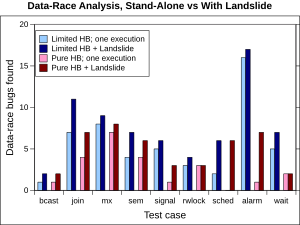
\includegraphics[width=0.8\textwidth]{../../oopsla/dr-false-negatives-poster.pdf}
	\end{center}
\end{frame}
\begin{frame}{Quicksand results - Representative of real-world programs?}
	Bugs by required number of preemptions to expose:
	\begin{center}
		\footnotesize
	\begin{tabular}{r|c|c}
		{\bf Bound} & {\bf SSS (sync PPs only)} & {\bf SSS (preempt everywhere)} \\
		\hline
		0       & 2     & 1     \\
		1       & 82    & 86    \\
		2       & 16    & 32    \\
		3       & 2     & 3     \\
		4+      & 0     & 0     \\
		\hline
		Total   & 102   & 122   \\
	\end{tabular}
	\end{center}
	\linegap

	Bugs by type (Pure HB trial):
	\begin{itemize}
		\item 56 deadlocks
		\item 49 heap errors (47 use-after-free)
		\item 35 assertion failures
		\item 31 page fault crashes
		\item 1 infinite loop
		\item 1 recursive mutex lock
	\end{itemize}
\end{frame}

% TODO: slide number c.c
\begin{frame}{Don't you need \texttt{if (mutex\_held(\&foo\_lock)) \_xabort();} in that transaction on slide 31?}
	Yes.
\end{frame}

\begin{frame}{References}
	\small
	\begin{itemize}
		\item {\bf [Lamport '78]}:
			Leslie Lamport. Time, clocks, and the ordering of events in a distributed system.
			Commun. ACM, 1978.
		\item {\bf [Godefroid '97]}: Patrice Godefroid.
			VeriSoft. A tool for the automatic analysis of concurrent reactive software. CAV 1997.
		%\item {\bf [Holzmann '97]}: The model checker SPIN. TOSE 1997.
		\item {\bf [Engler '03]}: Dawson Engler and Ken Ashcraft.
			RacerX: effective, static detection of race conditions and deadlocks. SOSP 2003.
		\item {\bf [O'Callahan '03]}: Robert O'Callahan and Jong-Deok Choi.
			Hybrid dynamic data race detection. PPoPP '03.
		\item {\bf [Flanagan '05]}: Cormac Flanagan and Patrice Godefroid. Dynamic partial-order reduction for
			model checking software. POPL 2005.
		\item {\bf [Musuvathi '08]}: Madanlal Musuvathi et al. Finding and Reproducing Heisenbugs in Concurrent
			Programs. OSDI 2008.
		\item {\bf [Yang '08]}: Yu Yang et al. Efficient stateful dynamic partial order reduction. SPIN 2008.
	\end{itemize}
\end{frame}
\begin{frame}{References}
	\small
	\begin{itemize}
		\item {\bf [Buckhardt '10]}: A randomized scheduler with probabilistic guarantees of finding bugs. ASPLOS 2010.
		\item {\bf [Simsa '12]}: Jiri Simsa. Runtime Estimation and Resource Allocation for
			Concurrency Testing. CMU-PDL-12-113. December 2012.
		\item {\bf [Blum '12]}: Ben Blum. Landslide: Systematic Dynamic Race Detection in Kernel
			Space. CMU-CS-12-118. May 2012.
		\item {\bf [Kasicki '12]}: Baris Kasicki. Data races vs. data race bugs: telling the difference with Portend. ASPLOS '12.
		\item {\bf [Huang '15]}: Jeff Huang. Stateless model checking concurrent programs with maximal causality reduction. PLDI '15.
		\item {\bf [Jensen '15]}: Stateless Model Checking of Event-Driven Applications. OOPSLA 2015.
	\end{itemize}
\end{frame}

\end{document}
